\documentclass[12pt,onecolumn]{article}
\usepackage[utf8]{inputenc} % UTF8 input encoding
\usepackage[T2A]{fontenc}   % T2A font encoding for Cyrillic script
\usepackage[russian]{babel} % Russian language support
\usepackage{listings}
\usepackage{float}
\usepackage{mathtools}
\everymath{\displaystyle}
\usepackage{listings} 
\usepackage[usenames]{color}
\usepackage{hyperref}
\usepackage{geometry}
\usepackage{verbatim}
\usepackage{framed}
\usepackage{amsmath}
\usepackage{tcolorbox}
\usepackage{pdfpages}
\usepackage{graphicx}
\usepackage[dvipsnames]{xcolor}
\usepackage{svg}
\usepackage{tabularx}
\usepackage{multirow}
\usepackage{graphicx}
\newcommand{\nparagraph}[1]{\paragraph{#1}\mbox{}\\}
\geometry{
  a4paper,
  top=20mm, 
  right=20mm, 
  bottom=20mm, 
  left=25mm
}
\lstdefinestyle{listing}{language=Python, 
  basicstyle=\small\ttfamily,
  commentstyle=\color{cyan},
  stringstyle=\color{magenta}\ttfamily,
  keywordstyle=\color{blue},
  numbers=left,
  numberstyle=\scriptsize,
  numbersep=5pt,
  frame=single,
  breaklines=true,
  breakatwhitespace=true,
  showstringspaces=false,
  tabsize=4,
  inputencoding=utf8,
  extendedchars=true,
  literate={ε}{{$\epsilon$}}1 {→}{{$\rightarrow$}}1
}

% Define a command to highlight text with a blue background
\newcommand{\hlb}[1]{
  \colorbox{Cyan}{#1}
}

% Define a command to highlight text with a lime green background
\newcommand{\hlg}[1]{
  \colorbox{LimeGreen}{#1}
}

% Define a command to highlight text with a pink background
\newcommand{\hlp}[1]{
  \colorbox{Lavender}{#1}
}

% Define a command to highlight text with a red background
\newcommand{\hlr}[1]{
  \colorbox{Salmon}{#1}
}

% Define a command to highlight text with a yellow background
\newcommand{\hly}[1]{
  \colorbox{Goldenrod}{#1}
}

% Define a command to highlight text with a orange background
\newcommand{\hlo}[1]{
  \colorbox{BurntOrange}{#1}
}

% Command: \chtb
% Description: Creates a centered table with two columns, where the first column contains the expression specified by the argument #3, and the second column contains the expression specified by the argument #4. The table width is determined by the argument #1.
% Parameters:
%   - #1: The width of the table (e.g., \textwidth, 0.8\linewidth)
%   - #2: The title of the table
%   - #3: The expression to be displayed in the first column
%   - #4: The expression to be displayed in the second column
\newcommand{\chtb}[4]{
  \begin{center}
    \textbf{#2}
  \end{center}
  \begin{center}
    \begin{tabularx}{#1}{X|X}
    $\begin{aligned}
          #3
      \end{aligned}$ &
    \begin{minipage}{1em}
      $\Rightarrow$
    \end{minipage}
    $\begin{aligned}
         #4
      \end{aligned}$
    \end{tabularx}
  \end{center}
}



\begin{document}
\setcounter{tocdepth}{4}
\begin{center}
    Федеральное государственное автономное образовательное учреждение высшего образования "Национальный Исследовательский Университет ИТМО"\\
    Мегафакультет Компьютерных Технологий и Управления\\
    Факультет Программной Инженерии и Компьютерной Техники \\
    
\includegraphics[scale=0.3]{image/itmo.jpg} % нужно закинуть картинку логтипа в папку с отчетом
\end{center}
\vspace{1cm}


\begin{center}
    \large \textbf{Вариант №5}\\
    \textbf{Домашняя работа 3}\\
    по дисциплине\\
    \textbf{'Разработка компиляторов'}
\end{center}

\vspace{2cm}

\begin{flushright}
    Выполнил Студент  группы P33102\\
    \textbf{Лапин Алексей Александрович}\\
    Преподаватель: \\
    \textbf{Лаздин Артур Вячеславович}\\
\end{flushright}

\vspace{9cm}
\begin{center}
    г. Санкт-Петербург\\
    2024г.
\end{center}
\pagestyle{empty}


\section*{Задание}
Задание к лабораторной (домашней) работе  «Конструирование LL(1) анализатора для КС-грамматики.»
Для грамматики из соответствующего варианта необходимо:
\begin{enumerate}
    \item Устранить левую рекурсию.
    \item Провести левую факторизацию грамматики.
    \item Для полученной преобразованной грамматики построить множества FIRST и\\ FOLLOW для нетерминальных символов грамматики.
    \item Для преобразованной грамматики реализовать синтаксический анализатор и реализовать программную реализацию этого анализатора.
    \item {
          Отчет должен включать:
          \begin{enumerate}
              \item Исходную грамматику;
              \item Отдельно (для каждого правила) действия по устранению прямой левой рекурсии и отдельно действия для левой факторизации.
              \item Преобразованную грамматику
              \item Таблицы множеств FIRST и FOLLOW для нетерминалов;
              \item Таблица синтаксического анализатора;
              \item Реализацию синтаксического анализатора.
              \item Выводы.
          \end{enumerate}
          }

\end{enumerate}
\begin{center}
    \fbox{
        \begin{minipage}{13em}
            \begin{tabularx}{\textwidth}{X}
                \textbf{Исходная грамматика} \\
                $\begin{aligned}
                          & \mathrm{S} \rightarrow \mathrm{A B B C}                                                \\
                          & \mathrm{B} \rightarrow \mathrm{b A}\mid \mathrm{b B} \mid \mathrm{b C} \mid \mathrm{b} \\
                          & \mathrm{C} \rightarrow \mathrm{CCa}\mid \mathrm{Ca}\mid \mathrm{a} \mid \mathrm{c}     \\
                          & \mathrm{A} \rightarrow \mathrm{aA} \mid \mathrm{aa}                                    \\
                     \end{aligned}$
            \end{tabularx}
        \end{minipage}
    }
\end{center}

\section*{Устранение левой рекурсии}

\begin{equation*}
    \mathrm{\hlr{C}} \rightarrow \mathrm{\hlr{C}Ca}\mid \mathrm{\hlr{C}a}\mid \mathrm{a} \mid \mathrm{c} \Rightarrow
    \left\{
    \begin{array}{l}
        \mathrm{C} \to \mathrm{a} \mid \mathrm{c} \mid \mathrm{aD} \mid \mathrm{cD}   \\
        \mathrm{D} \to \mathrm{Ca} \mid \mathrm{a} \mid \mathrm{CaD} \mid \mathrm{aD} \\
    \end{array}
    \right.
\end{equation*}

\chtb{0.7\textwidth}
{Стало:}
{
    & \mathrm{S} \rightarrow \mathrm{A B B C}                                                \\
    & \mathrm{B} \rightarrow \mathrm{b A}\mid \mathrm{b B} \mid \mathrm{b C} \mid \mathrm{b} \\
    & \mathrm{C} \rightarrow \mathrm{CCa}\mid \mathrm{Ca}\mid \mathrm{a} \mid \mathrm{c}    \\
    & \mathrm{A} \rightarrow \mathrm{aA} \mid \mathrm{aa}
}
{
    & \mathrm{S} \rightarrow \mathrm{A B B C}                                            \\
    & \mathrm{B} \rightarrow \mathrm{b A}\mid \mathrm{b B} \mid \mathrm{b C} \mid \mathrm{b} \\
    & \mathrm{C} \rightarrow \mathrm{a} \mid \mathrm{c} \mid \mathrm{aD} \mid \mathrm{cD} \\
    & \mathrm{D} \rightarrow \mathrm{Ca} \mid \mathrm{a} \mid \mathrm{CaD} \mid \mathrm{aD} \\
    & \mathrm{A} \rightarrow \mathrm{aA} \mid \mathrm{aa}
}

\section*{Левая факторизация}
\begin{center}
    \fbox{
        \begin{minipage}{15em}
            \begin{enumerate}
                \item[] $\mathrm{S} \rightarrow \mathrm{A B B C}$
                \item[] $\mathrm{B} \rightarrow \mathrm{\hlb{b}A}\mid \mathrm{\hlb{b} B} \mid \mathrm{\hlb{b} C} \mid \mathrm{\hlb{b}}$
                \item[] $\mathrm{C} \to \mathrm{\hlg{a}} \mid \mathrm{\hlp{c}} \mid \mathrm{\hlg{a}D} \mid \mathrm{\hlp{c}D}$
                \item[] $\mathrm{D} \to \mathrm{\hlr{Ca}} \mid \mathrm{\hly{a}} \mid \mathrm{\hlr{Ca}D} \mid \mathrm{\hly{a}D}$
                \item[] $\mathrm{A} \rightarrow \mathrm{\hlo{a}A} \mid \mathrm{\hlo{a}a}$
            \end{enumerate}
        \end{minipage}
    }
\end{center}

$
    \mathrm{B} \rightarrow \mathrm{\hlb{b}A}\mid \mathrm{\hlb{b} B} \mid \mathrm{\hlb{b} C} \mid \mathrm{\hlb{b}}
    \Rightarrow
    \left\{
    \begin{array}{l}
        \mathrm{B} \rightarrow \mathrm{\hlb{b}E} \\
        \mathrm{E} \rightarrow \mathrm{A} \mid \mathrm{B} \mid \mathrm{C} \mid \varepsilon
    \end{array}
    \right.
$

$
    \mathrm{A} \rightarrow \mathrm{\hlo{a}A} \mid \mathrm{\hlo{a}a}
    \Rightarrow
    \left\{
    \begin{array}{l}
        \mathrm{A} \rightarrow \mathrm{\hlo{a}F} \\
        \mathrm{F} \rightarrow \mathrm{A} \mid \mathrm{a}
    \end{array}
    \right.
$

$
    \mathrm{C} \to \mathrm{\hlg{a}} \mid \mathrm{\hlp{c}} \mid \mathrm{\hlg{a}D} \mid \mathrm{\hlp{c}D}
    \Rightarrow
    \left\{
    \begin{array}{l}
        \mathrm{C} \to \mathrm{\hlg{a}G} \mid \mathrm{\hlp{c}} \mid \mathrm{\hlp{c}D} \\
        \mathrm{G} \to \mathrm{D} \mid \varepsilon
    \end{array}
    \right.
    \Rightarrow
    \left\{
    \begin{array}{l}
        \mathrm{C} \to \mathrm{\hlg{a}G} \mid \mathrm{\hlp{c}I} \\
        \mathrm{G} \to \mathrm{D} \mid \varepsilon              \\
        \mathrm{I} \to \mathrm{D} \mid \varepsilon
    \end{array}
    \right.
$

$
    \mathrm{D} \to \mathrm{\hlr{Ca}} \mid \mathrm{\hly{a}} \mid \mathrm{\hlr{Ca}D} \mid \mathrm{\hly{a}D}
    \Rightarrow
    \left\{
    \begin{array}{l}
        \mathrm{D} \to \mathrm{\hlr{Ca}H} \mid \mathrm{\hly{a}} \mid \mathrm{\hly{a}D} \\
        \mathrm{H} \to \mathrm{D} \mid \varepsilon
    \end{array}
    \right.
    \Rightarrow
    \left\{
    \begin{array}{l}
        \mathrm{D} \to \mathrm{\hlr{Ca}J} \mid \mathrm{\hly{a}J} \\
        \mathrm{H} \to \mathrm{D} \mid \varepsilon               \\
        \mathrm{J} \to \mathrm{D} \mid \varepsilon
    \end{array}
    \right.
$


\begin{center}
    \textbf{Уберем эквивалентные правила:}\\[1em]
    \begin{tabularx}{0.6\textwidth}{X|X}
        Исходные правила:                                &
        Упрощенное правило:                                \\
        $\begin{aligned}
                  & \mathrm{G} \to \mathrm{D} \mid \varepsilon \\
                  & \mathrm{I} \to \mathrm{D} \mid \varepsilon \\
                  & \mathrm{H} \to \mathrm{D} \mid \varepsilon \\
                  & \mathrm{J} \to \mathrm{D} \mid \varepsilon
             \end{aligned}$ &
        $\begin{aligned}
                  & \mathrm{G} \to \mathrm{D} \mid \varepsilon
             \end{aligned}$
    \end{tabularx}
\end{center}



\chtb{0.6\textwidth}
{Стало:}
{
    & \mathrm{S} \rightarrow \mathrm{A B B C}                                                \\
    & \mathrm{B} \rightarrow \mathrm{b A}\mid \mathrm{b B} \mid \mathrm{b C} \mid \mathrm{b} \\
    & \mathrm{C} \to \mathrm{a} \mid \mathrm{c} \mid \mathrm{aD} \mid \mathrm{cD}            \\
    & \mathrm{D} \to \mathrm{Ca} \mid \mathrm{a} \mid \mathrm{CaD} \mid \mathrm{aD}          \\
    & \mathrm{A} \rightarrow \mathrm{aA} \mid \mathrm{aa}
}
{
    & \mathrm{S} \rightarrow \mathrm{A B B C}                                            \\
    & \mathrm{B} \rightarrow \mathrm{b E}                                                \\
    & \mathrm{E} \rightarrow \mathrm{A} \mid \mathrm{B} \mid \mathrm{C} \mid \varepsilon \\
    & \mathrm{C} \to \mathrm{aG} \mid \mathrm{cG}                                        \\
    & \mathrm{D} \to \mathrm{CaG} \mid \mathrm{aG}                                       \\
    & \mathrm{G} \to \mathrm{D} \mid \varepsilon                                         \\
    & \mathrm{A} \rightarrow \mathrm{aF}                                                 \\
    & \mathrm{F} \rightarrow \mathrm{A} \mid \mathrm{a}
}


\section*{Множества FIRST и FOLLOW}
\fbox{
    \begin{minipage}{\textwidth}
        \begin{center}
            \textbf{FIRST \& FOLLOW}\\[1em]
            \begin{tabularx}{\textwidth}{X|X|X}
                \textbf{Грамматика:}                                                           &
                \textbf{FIRST}                                                                 &
                \textbf{FOLLOW}                                                                  \\
                $\begin{aligned}
                          & \mathrm{S} = \mathrm{ABBC}                                               \\
                          & \mathrm{B} = \mathrm{bE}                                                 \\
                          & \mathrm{E} = \mathrm{A} \mid \mathrm{B} \mid \mathrm{C} \mid \varepsilon \\
                          & \mathrm{C} = \mathrm{aG} \mid \mathrm{cG}                                \\
                          & \mathrm{D} = \mathrm{CaG} \mid \mathrm{aG}                               \\
                          & \mathrm{G} = \mathrm{D} \mid \varepsilon                                 \\
                          & \mathrm{A} = \mathrm{aF}                                                 \\
                          & \mathrm{F} = \mathrm{A} \mid \mathrm{a}
                     \end{aligned}$ &
                $\begin{aligned}
                          & \mathrm{FIRST(S)} = \{ \mathrm{a} \}                    \\
                          & \mathrm{FIRST(B)} = \{ \mathrm{b} \}                    \\
                          & \mathrm{FIRST(E)} = \{ \mathrm{a, b, c, \varepsilon} \} \\
                          & \mathrm{FIRST(C)} = \{ \mathrm{a, c} \}                 \\
                          & \mathrm{FIRST(D)} = \{ \mathrm{a, c} \}                 \\
                          & \mathrm{FIRST(G)} = \{ \mathrm{a, c, \varepsilon} \}    \\
                          & \mathrm{FIRST(A)} = \{ \mathrm{a} \}                    \\
                          & \mathrm{FIRST(F)} = \{ \mathrm{a} \}                    \\
                     \end{aligned}$                  &
                $\begin{aligned}
                          & \mathrm{FOLLOW(S)} = \{ \$ \}                                    \\
                          & \mathrm{FOLLOW(B)} = \{ \mathrm{a}, \mathrm{b}, \mathrm{c}\}     \\
                          & \mathrm{FOLLOW(E)} = \{ \mathrm{a}, \mathrm{b}, \mathrm{c}\}     \\
                          & \mathrm{FOLLOW(C)} = \{ \$, \mathrm{a}, \mathrm{b}, \mathrm{c}\} \\
                          & \mathrm{FOLLOW(D)} = \{ \$, \mathrm{a}, \mathrm{b}, \mathrm{c}\} \\
                          & \mathrm{FOLLOW(G)} = \{ \$, \mathrm{a}, \mathrm{b}, \mathrm{c}\} \\
                          & \mathrm{FOLLOW(A)} = \{ \mathrm{a}, \mathrm{b}, \mathrm{c}\}     \\
                          & \mathrm{FOLLOW(F)} = \{ \mathrm{a}, \mathrm{b}, \mathrm{c}\}     \\
                     \end{aligned}$
            \end{tabularx}
        \end{center}
    \end{minipage}
}

\begin{center}
    \begin{tabularx}{0.7\textwidth}{X}
        \vspace{1em}
        $\ast$~$\ast$~$\ast$ \\[1em]
        $\begin{aligned}
                  & \mathrm{FIRST\left(S\right)} = \mathrm{FIRST\left(A\right)} = \{ \mathrm{a} \} \\
                  & \mathrm{FIRST\left(B\right)} = \{b \}                                          \\
                  & \mathrm{FIRST\left(E\right)} =
                 \left\{
                 \begin{array}{l}
                    \mathrm{FIRST\left(A\right)} = \mathrm{a}    \\
                    \mathrm{FIRST\left(B\right)} = b             \\
                    \mathrm{FIRST\left(C\right)} = \mathrm{a, c} \\
                    \varepsilon
                \end{array}
                 \right.
                 = \{ \mathrm{a, b, c, \varepsilon}  \}                                            \\
                  & \mathrm{FIRST\left(C\right)} = \{ \mathrm{a, c}   \}                           \\
                  & \mathrm{FIRST\left(D\right)} =  \left\{
                 \begin{array}{l}
                    \mathrm{FIRST\left(C\right)} = \{ \mathrm{a, c}   \} \\
                    a
                \end{array}
                 \right. = \{ \mathrm{a, c} \}                                                     \\
                  & \mathrm{FIRST\left(G\right)} = \left\{
                 \begin{array}{l}
                    \mathrm{FIRST\left(D\right)} = \{ \mathrm{a, c} \} \\
                    \varepsilon
                \end{array}
                 \right. = \{ \mathrm{a, c, \varepsilon} \}                                        \\
                  & \mathrm{FIRST\left(A\right)} = \{ \mathrm{a} \}                                \\
                  & \mathrm{FIRST\left(F\right)} = \left\{
                 \begin{array}{l}
                    \mathrm{FIRST\left(A\right)} = \{ \mathrm{a} \} \\
                    a
                \end{array}
                 \right. = \{ \mathrm{a} \}
             \end{aligned}$

        \vspace{1em}
        $\ast$~$\ast$~$\ast$ \\[1em]
        $\begin{aligned}
                  & \mathrm{FOLLOW\left(S\right)} = \{ \$ \}                                                                     \\
                  & \mathrm{FOLLOW\left(B\right)} =
                 \left\{
                 \begin{array}{l}
                    \mathrm{FIRST\left(B\right)} = \{ \mathrm{b} \} \\
                    \mathrm{FOLLOW\left(E\right)} = \{ \mathrm{a}, \mathrm{b}, \mathrm{c}\}
                \end{array}
                 \right. = \{ \mathrm{a}, \mathrm{b}, \mathrm{c} \}                                                              \\
                  & \mathrm{FOLLOW\left(E\right)} = \mathrm{FOLLOW\left(B\right)} = \{ \mathrm{a}, \mathrm{b}, \mathrm{c} \}     \\
                  & \mathrm{FOLLOW\left(C\right)} =
                 \left\{
                 \begin{array}{l}
                    \mathrm{FOLLOW\left(S\right)} = \{ \$ \} \\
                    \mathrm{FOLLOW\left(E\right)} = \{ \mathrm{a}, \mathrm{b}, \mathrm{c} \}
                \end{array}
                 \right.
                 = \{ \$, \mathrm{a}, \mathrm{b}, \mathrm{c} \}                                                                  \\
                  & \mathrm{FOLLOW\left(D\right)} = \mathrm{FOLLOW\left(G\right)} = \{ \$, \mathrm{a}, \mathrm{b}, \mathrm{c} \} \\
                  & \mathrm{FOLLOW\left(G\right)} = \mathrm{FOLLOW\left(C\right)} = \{ \$, \mathrm{a}, \mathrm{b}, \mathrm{c} \} \\
                  & \mathrm{FOLLOW\left(A\right)} = \left\{
                 \begin{array}{l}
                    \mathrm{FIRST\left(B\right)} = \{ \mathrm{b} \} \\
                    \mathrm{FOLLOW\left(E\right)} = \{ \mathrm{a}, \mathrm{b}, \mathrm{c} \}
                \end{array}
                 \right.
                 = \{ \mathrm{a}, \mathrm{b}, \mathrm{c} \}                                                                      \\
                  & \mathrm{FOLLOW\left(F\right)} = \mathrm{FOLLOW\left(A\right)} = \{ \mathrm{a}, \mathrm{b}, \mathrm{c} \}
             \end{aligned}$
    \end{tabularx}
\end{center}
\newpage
\textbf{Множество Nullable}
\begin{table}[H]
    \centering
    \resizebox{\textwidth}{!}{%
        \begin{tabular}{|l|l|l|l|l|l|l|l|}
            \hline
            A     & B     & C     & D     & E             & F     & G             & S     \\ \hline
            FALSE & FALSE & FALSE & FALSE & \textbf{TRUE} & FALSE & \textbf{TRUE} & FALSE \\ \hline
        \end{tabular}%
    }
\end{table}
\section*{Таблица синтаксического анализатора}
\begin{table}[H]
    \centering
    \resizebox{\textwidth}{!}{%
        \begin{tabular}{|l|llll|}
            \hline
            \multirow{2}{*}{NTs} & \multicolumn{4}{l|}{Input Symbols}                                                                                                                                                                                                                                                  \\ \cline{2-5}
                                 & \multicolumn{1}{l|}{a}                                                                      & \multicolumn{1}{l|}{b}                                                   & \multicolumn{1}{l|}{c}                                                   & \$                              \\ \hline
            $\mathrm{S}$         & \multicolumn{1}{l|}{$ \mathrm{S}   \to  \mathrm{ABBC} $ }                                   & \multicolumn{1}{l|}{}                                                    & \multicolumn{1}{l|}{}                                                    &                                 \\ \hline
            $\mathrm{B}$         & \multicolumn{1}{l|}{}                                                                       & \multicolumn{1}{l|}{$ \mathrm{B}   \to  \mathrm{bE} $ }                  & \multicolumn{1}{l|}{}                                                    &                                 \\ \hline
            $\mathrm{E}$         & \multicolumn{1}{l|}{$ \mathrm{E}   \to  \mathrm{A}   \mid  \mathrm{C}   \mid  \varepsilon$} & \multicolumn{1}{l|}{$ \mathrm{E}   \to  \mathrm{B}   \mid  \varepsilon$} & \multicolumn{1}{l|}{$ \mathrm{E}   \to  \mathrm{C}   \mid  \varepsilon$} &                                 \\ \hline
            $\mathrm{C}$         & \multicolumn{1}{l|}{$ \mathrm{C}   \to  \mathrm{aG} $ }                                     & \multicolumn{1}{l|}{}                                                    & \multicolumn{1}{l|}{$ \mathrm{C}   \to  \mathrm{cG} $ }                  &                                 \\ \hline
            $\mathrm{D}$         & \multicolumn{1}{l|}{$ \mathrm{D}   \to  \mathrm{CaG}   \mid   \mathrm{aG} $ }               & \multicolumn{1}{l|}{}                                                    & \multicolumn{1}{l|}{$ \mathrm{D}   \to  \mathrm{CaG} $ }                 &                                 \\ \hline
            $\mathrm{G}$         & \multicolumn{1}{l|}{$ \mathrm{G}   \to  \mathrm{D}   \mid  \varepsilon$}                    & \multicolumn{1}{l|}{$ \mathrm{G}   \to \varepsilon$}                     & \multicolumn{1}{l|}{$ \mathrm{G}   \to  \mathrm{D}   \mid  \varepsilon$} & $ \mathrm{G}   \to \varepsilon$ \\ \hline
            $\mathrm{A}$         & \multicolumn{1}{l|}{$ \mathrm{A}   \to  \mathrm{aF} $ }                                     & \multicolumn{1}{l|}{}                                                    & \multicolumn{1}{l|}{}                                                    &                                 \\ \hline
            $\mathrm{F}$         & \multicolumn{1}{l|}{$ \mathrm{F}   \to  \mathrm{A}   \mid   \mathrm{a} $ }                  & \multicolumn{1}{l|}{}                                                    & \multicolumn{1}{l|}{}                                                    &                                 \\ \hline
        \end{tabular}%
    }
\end{table}

Так как A для пары (X, c) применимо более
одного правила, то это не LL(1)
грамматика.

Насильно преобразуем к LL(1).

Удаляем правила:

$\begin{aligned}
         & \mathrm{E} \to \mathrm{C} \mid \varepsilon   \\
         & \mathrm{D} \to \mathrm{CaG} \mid \varepsilon \\
         & \mathrm{G} \to  \mathrm{D}                   \\
         & \mathrm{F} \to \mathrm{A} \mid \varepsilon
    \end{aligned}$

Грамматика:

$\begin{aligned}
         & \mathrm{S} \to \mathrm{ABBC}                \\
         & \mathrm{B} \to \mathrm{bE}                  \\
         & \mathrm{E} \to  \mathrm{A}  \mid \mathrm{b} \\
         & \mathrm{C} \to \mathrm{a} \mid \mathrm{c}   \\
         & \mathrm{A} \to \mathrm{aF}                  \\
         & \mathrm{F} \to \mathrm{a}                   \\
    \end{aligned}$

\fbox{
    \begin{minipage}{\textwidth}
        \begin{center}
            \textbf{FIRST \& FOLLOW}\\[1em]
            \begin{tabularx}{\textwidth}{X|X|X}
                \textbf{Грамматика:}                              &
                \textbf{FIRST}                                    &
                \textbf{FOLLOW}                                     \\
                $\begin{aligned}
                          & \mathrm{S} \to \mathrm{ABBC}                \\
                          & \mathrm{A} \to \mathrm{aF}                  \\
                          & \mathrm{B} \to \mathrm{bE}                  \\
                          & \mathrm{C} \to \mathrm{a} \mid \mathrm{c}   \\
                          & \mathrm{E} \to  \mathrm{A}  \mid \mathrm{B} \\
                          & \mathrm{F} \to \mathrm{a}                   \\
                     \end{aligned}$ &
                $\begin{aligned}
                          & \mathrm{FIRST(S)} = \{ \mathrm{a} \}    \\
                          & \mathrm{FIRST(A)} = \{ \mathrm{a} \}    \\
                          & \mathrm{FIRST(B)} = \{ \mathrm{b} \}    \\
                          & \mathrm{FIRST(C)} = \{ \mathrm{a, c} \} \\
                          & \mathrm{FIRST(E)} = \{ \mathrm{a, b} \} \\
                          & \mathrm{FIRST(F)} = \{ \mathrm{a} \}    \\
                     \end{aligned}$     &
                $\begin{aligned}
                          & \mathrm{FOLLOW(S)} = \{ \$ \}                                \\
                          & \mathrm{FOLLOW(A)} = \{ \mathrm{a}, \mathrm{b}, \mathrm{c}\} \\
                          & \mathrm{FOLLOW(B)} = \{ \mathrm{a}, \mathrm{b}, \mathrm{c}\} \\
                          & \mathrm{FOLLOW(C)} = \{ \$\}                                 \\
                          & \mathrm{FOLLOW(E)} = \{ \mathrm{a}, \mathrm{b}, \mathrm{c}\} \\
                          & \mathrm{FOLLOW(F)} = \{ \mathrm{a}, \mathrm{b}, \mathrm{c}\} \\
                     \end{aligned}$
            \end{tabularx}
        \end{center}
    \end{minipage}
}

% Please add the following required packages to your document preamble:
% \usepackage{multirow}
\begin{table}[H]
    \begin{tabular}{|l|llll|}
        \hline
        \multirow{2}{*}{NTs} & \multicolumn{4}{l|}{Input Symbols}                                                                         \\ \cline{2-5}
                             & \multicolumn{1}{l|}{a}             & \multicolumn{1}{l|}{b}          & \multicolumn{1}{l|}{c}         & \$ \\ \hline
        S                    & \multicolumn{1}{l|}{$S \to ABBC$}  & \multicolumn{1}{l|}{}           & \multicolumn{1}{l|}{}          &    \\ \hline
        B                    & \multicolumn{1}{l|}{}              & \multicolumn{1}{l|}{$B \to bE$} & \multicolumn{1}{l|}{}          &    \\ \hline
        E                    & \multicolumn{1}{l|}{$E \to A $}    & \multicolumn{1}{l|}{$E \to b $} & \multicolumn{1}{l|}{}          &    \\ \hline
        C                    & \multicolumn{1}{l|}{$C \to a$}     & \multicolumn{1}{l|}{}           & \multicolumn{1}{l|}{$C \to c$} &    \\ \hline
        A                    & \multicolumn{1}{l|}{$A \to aF$}    & \multicolumn{1}{l|}{}           & \multicolumn{1}{l|}{}          &    \\ \hline
        F                    & \multicolumn{1}{l|}{$F \to  a$}    & \multicolumn{1}{l|}{}           & \multicolumn{1}{l|}{}          &    \\ \hline
    \end{tabular}
\end{table}
\section*{Программа-распознаватель}
\subsection*{Код}
\lstinputlisting[style=listing]{./main.py}
\subsection*{Вывод}
\begin{figure}[H]
    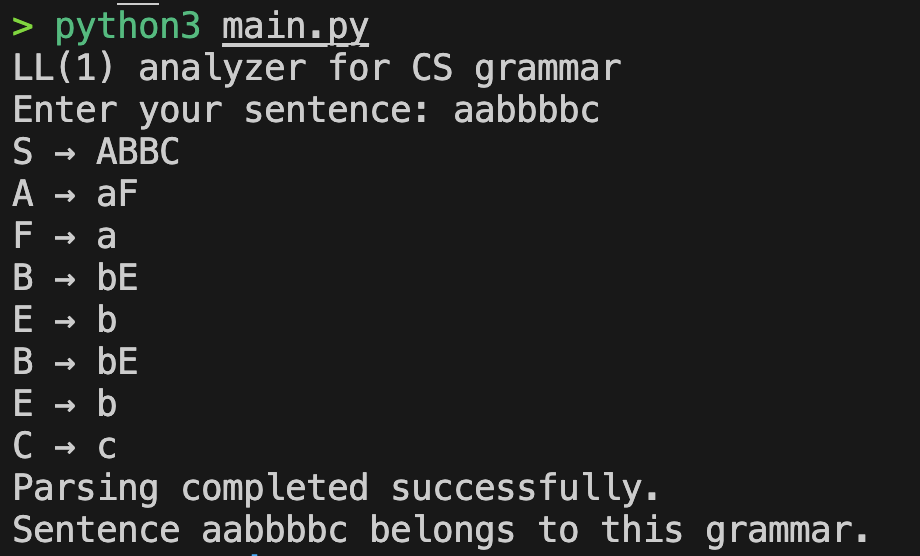
\includegraphics[width=\textwidth]{image/out1.png}
\end{figure}
\begin{figure}[H]
    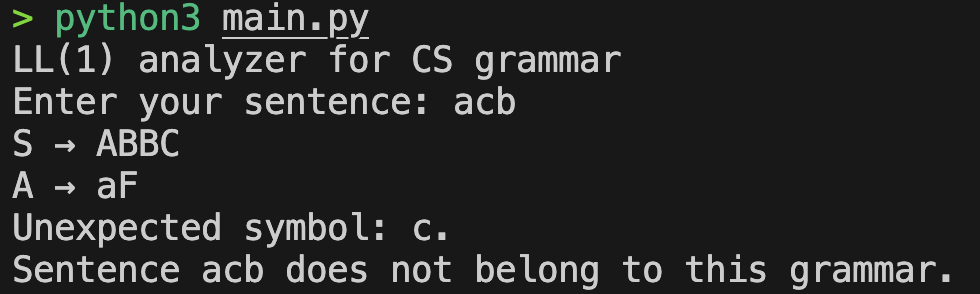
\includegraphics[width=\textwidth]{image/out2.png}
\end{figure}



\end{document}